\documentclass[12pt,oneside]{article}
\usepackage[english,russian]{babel}
\usepackage[utf8]{inputenc}
\usepackage[T2A]{fontenc}
\usepackage{csquotes}
\usepackage{bookmark}
\usepackage{setspace}
  \setstretch{1.05}
\usepackage[style=authoryear,sorting=nyt,backend=biber,
  hyperref=true,abbreviate=true,
  maxcitenames=1,maxbibnames=1]{biblatex}
  \renewbibmacro{in:}{}
  \addbibresource{../main.bib}
\usepackage{xcolor}
  \definecolor{dgreen}{RGB}{62,100,62}
  \definecolor{lgreen}{RGB}{249,255,249}
  \pagecolor{lgreen}
\usepackage{graphicx}
\usepackage{hyperref}
  \hypersetup{colorlinks=true,allcolors=blue!40!black}
\setlength{\topskip}{6pt}
\setlength{\parskip}{6pt} % before par

\DeclareCiteCommand{\citea}
  {\boolfalse{citetracker}\boolfalse{pagetracker}\usebibmacro{prenote}}
  {\href{\thefield{url}}{\printnames{labelname}}}
  {\multicitedelim}
  {\usebibmacro{postnote}}

\def\zoldversion{0.2.4}

\title{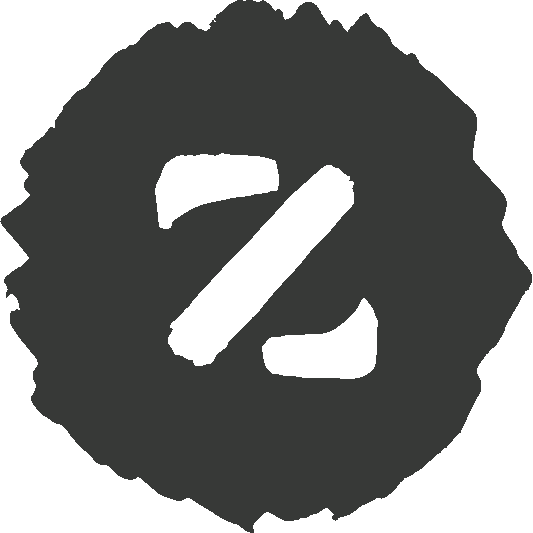
\includegraphics[scale=0.3]{../images/logo.pdf}\\
  Zold: Новая Криптовалюта\\
  {\small\colorbox{dgreen}{\color{lgreen}{Green Paper}}}}
\author{Yegor Bugayenko\\
  \texttt{yegor256@gmail.com}\\
  \href{https://www.zold.io}{\texttt{www.zold.io}}\\[1em]
  \href{https://github.com/zold-io/papers/releases/tag/\zoldversion}{\texttt{\zoldversion}}}

\begin{document}
\raggedbottom

\maketitle

За последние несколько лет цифровые валюты успешно продемонстрировали свою
способность стать альтернативным финансовым инструментом на различных рынках.
Большая часть доступных в данный момент технологий построена на принципах
архитектуры \href{https://en.wikipedia.org/wiki/Blockchain}{Blockchain},
туда можно отнести такие распространенные валюты как
\href{https://bitcoin.org/}{Bit\-coin} и \href{https://ethereum.org/}{Ethe\-reum}.
Несмотря на свою популярность, Blockchain --- хорошее решение
не для всех ситуаций. Один из примеров таких ситуаций --- быстрые микротранзакции.
\href{https://www.zold.io}{Zold} --- экспериментальная альтернатива, которая делает возможными распределенные
транзакции между анонимными пользователями, которые делают микроплатежи более
финансово доступными и быстрыми. Zold заимствует принцип
«\href{https://ru.wikipedia.org/wiki/%D0%94%D0%BE%D0%BA%D0%B0%D0%B7%D0%B0%D1%82%D0%B5%D0%BB%D1%8C%D1%81%D1%82%D0%B2%D0%BE_%D0%B2%D1%8B%D0%BF%D0%BE%D0%BB%D0%BD%D0%B5%D0%BD%D0%B8%D1%8F_%D1%80%D0%B0%D0%B1%D0%BE%D1%82%D1%8B}{доказательства выполнения работы}»
у Bitcoin и предлагает другую архитектуру для обслуживания
цифровых кошельков, о чем подробнее рассказывается в
\href{https://papers.zold.io}{White Paper}.

\pagebreak

\section*{Рынок}

С момента выпуска в 2009 году, \href{https://bitcoin.org/}{Bitcoin} из «либертарианской сказки»
и «модного движения в Силиконовой Долине» превратился в «катализатор изменения финансовой
системы в пользу большей эффективности для физических лиц и фирм», пишет
\citea{andreessen2014}. Несмотря на заявление \citea{cheah2015} о том, что «фундаментальное значение
Bitcoin равняется нулю», \citea{van2014} утверждает: «Вопрос не в том, имеет ли
ценность Bitcoin; а он имеет. Важно то, может ли продуктивность такой
криптовалюты как Bitcoin соединиться с надежностью честного Центрального банка».

Основным компонентом Bitcoin является технология Blockchain, которая
«гарантирует устранение проблемы двойного расходования при помощи криптосистемы
с открытым ключом» и «деньги переводятся посредством электронной подписи в
хэше», объясняет \citea{pilkington2016}. Вскоре после того как создали Bitcoin, были
представлены подобные криптовалюты, также основанные на принципах Blockchain,
такие как \href{https://ethereum.org/}{Ethereum} от \citea{buterin2013}.

Несмотря на то, что Blockchain --- разумное решение проблемы
\href{https://ru.wikipedia.org/wiki/%D0%94%D0%B2%D0%BE%D0%B9%D0%BD%D0%BE%D0%B5_%D1%80%D0%B0%D1%81%D1%85%D0%BE%D0%B4%D0%BE%D0%B2%D0%B0%D0%BD%D0%B8%D0%B5}{двойного расходования},
существует множество других решений из разряда «доказательство Х».
К примеру, \citea{everaere2010} опубликовали по этим решениям краткий анализ и объявили
о создании своего варианта решения данной проблемы; \citea{boyen2016} описали
«действительно распределённую книгу учёта на основе плоского графика
кросс-проверочных операций»; недавно \href{https://www.iota.org/}{IOTA}, «криптовалюта на основе сплетений», была
запущена \citea{popov2017}; \citea{hashgraph} по их собственным словам
признана «первой в мире принятой в массах публичной
книгой учёта».

\pagebreak

\section*{Проблемы}

Zold является децентрализованной цифровой валютой, которая поддерживает свои
книги учёта посредством непредсказуемого количества анонимных и ненадежных
серверных нодов, стараясь гарантировать последовательность данных. Архитектура
Zold не основывается на принципах Blockchain. Разработка Zold была мотивирована желанием
обойти два очевидных недостатка, присутствующих в большинстве существующих
криптовалют:

Первая проблема состоит в том, что обработка транзакции довольно
медлительна. Скорость обработки Bitcoin
\href{https://goo.gl/sWiAWc}{в настоящий момент} --- семь транзакций в
секунду (tps), в то время как PayPal в среднем справляется со 115 tps, а сеть
VISA достигает предела в 47000 tps. \citea{karame2012} утверждает, что «Bitcoin
нуждается в десятках минут для подтверждения транзакции и, ввиду этого, не
подходит для быстрых платежей». Это неизбежно, поскольку «скорость обработки
напрямую зависит от механизма безопасности, обеспечивающего правильность работы»
отмечает \citea{kiayias2015}. По словам \citea{fekkes2018},
\href{https://ethereum.org/}{Ethereum} способен обрабатывать
«в два раза больше транзакций, чем Bitcoin», но в итоге это всё равно довольно
медленно.

Вторая проблема, как было замечено \citea{popov2017}, состоит в том, что «не так-то просто
избавиться от налогов в инфраструктуре Blockchain, поскольку они служат стимулом
для создателей блоков». \citea{moser2015} говорит, что «пользователям Bitcoin
предлагают платить налоги майнерам до 10 центов (в долларах США) за каждую
транзакцию вне зависимости от количества оплаты», что особенно ощутимо в случае,
когда сумма транзакции составляет менее одного доллара. Более того, по словам
\citea{kaskaloglu2014}, «увеличение в сумме налогов на транзакции Bitcoin неизбежно»,
Таким образом, скорость операций является низкой, а стоимость обработки ---
высокой. Zold была создана в качестве попытки решения этих двух проблем.

\pagebreak

\section*{Функции}

Во-первых, в отличие от всех других криптовалют, в Zold нет центральной
распределённой книги учёта. У каждого кошелька есть своя книга учёта. Все
операции в каждой из них подтверждаются
\href{https://ru.wikipedia.org/wiki/RSA}{RSA}-подпися\-ми владельцев кошельков. Это
делает возможными высокую производительность и масштабируемость базы данных.

Во-вторых, будучи схожей с иными цифровыми валютами, включая Bitcoin, Ethereum,
\href{https://getmonero.org/}{Monero}, \href{https://plancoin.co/}{Plancoin},
\href{https://dero.io/}{Dero} и другие, ноды Zold, используя силу CPU, затраченную
каждым из них на выполнение определённых «бессмысленных» вычислений,
находят консенсус, который приводит к нахождению хэш-суффиксов, которые также
известны как «доказательство проделанной работы», изначально представленное \citea{back1997}
в \citeyear{back1997}. Это гарантирует последовательность данных и устраняет возможность
появления проблемы двойного расходования.

В-третьих, Zold --- это цифровой премайн-актив, подобный \href{https://ripple.com/}{Ripple},
\href{https://www.cardano.org/en/home/}{Cardano},
\href{https://www.stellar.org/}{Stellar},
\href{https://neo.org/}{NEO} и другим криптовалютам. При помощи алгоритмов Zold ограничивает свой общий
запас монет объёмом в 2,15 млрд ZLD. Для сравнения, общий запас других
криптовалют составляет:
21 млн у \href{https://bitcoin.org/}{Bitcoin},
100 млрд у \href{https://ripple.com/}{Ripple},
84 млн у \href{https://litecoin.org/}{Litecoin},
и
19 млн у \href{https://www.dash.org/}{Dash}.
\citea{bohr2014} объясняет, что криптовалюты лимитируют свои запасы с
целью «защититься от сил инфляции»; то же самое делает и Zold, чтобы обезопасить
свою ценность на рынке.

В-четвертых, скорость выполняемых Zold операций буквально безгранична, так как
все платежи производятся локально на устройствах пользователей, а затем
направляются в сеть для соединения и хранения.

В-пятых, стоимость обработки транзакций у Zold значительно ниже, чем может
предложить большинство других платёжных систем. Чтобы обработать 1000
транзакций, пользователь должен заплатить около \$500 при работе с Bitcoin, \$300
с Ethereum, \$45 с \href{https://litecoin.org/}{Litecoin}, \$12 с \href{https://ripple.com/}{Ripple}
и \$9 с Bitcoin Cash. В работе с Zold
такое же количество операций обходится всего в \$4, что делает её одной из самых
финансово выгодных криптовалют.

\pagebreak

\section*{Стратегия}

Zold --- это размещённое на \href{https://github.com/zold-io}{GitHub} программное обеспечение с открытым исходным
кодом, равно как и многие другие криптовалюты. Её первая экспериментальная версия была
создана и запущена \href{https://www.yegor256.com}{Егором Бугаенко}, СЕО в \href{https://www.zerocracy.com}{Zerocracy}, 27 мая 2018 года.
Распределённая \href{http://www.zold.io/map.html}{сеть нодов}, которые управляют
программным обеспечением Zold, поддерживается анонимными
добровольцами. Разработка последующих версий и обслуживание имеющихся зависит от
того, насколько активно поддерживают проект участники GitHub, частично
финансируемые \href{https://www.zerocracy.com}{компанией Zerocracy}.

Как \href{https://www.cnbc.com/video/2018/06/06/sec-chairman-cryptocurrencies-like-bitcoin--not-securities.html}{недавно отметил}
председатель \href{https://www.sec.gov/}{SEC} Jay Clayton, «криптовалюты вроде Bitcoin ---
не ценные бумаги». Подобно Bitcoin и Ethereum, Zold --- это криптовалюта, а не
ценная бумага. Она раздается Zerocracy в качестве цифрового подарка тем, кто
активно сотрудничает с экосистемой Zerocracy, участвует в разработке программного обеспечения
Zold и занимается поддержкой нодов.

Кропе программирования, добровольцы могут внести свой денежный актив, например,
доллары США, в любой из проектов, разрабатываемых и руководимых Zerocracy.
Взамен, в качестве вознаграждения, они получают цифровые монеты ZLD. Далее, ZLD
можно поменять на другие криптовалюты и бумажные деньги посредством обмена на биржах.

Предполагается, что рыночная стоимость ZLD будет расти благодаря техническим
преимуществам и популярности платформы Zerocracy среди программистов и
программных компаний.

\end{document}
